%1. La memoria incluirá una portada portada normalizada con la siguiente información: título en castellano, título en inglés, autores, profesor director, codirector si es el caso, curso académico e identificación de la asignatura (Trabajo de fin de grado del Grado en - nombre del grado correspondiente-, Facultad de Informática, Universidad Complutense de Madrid). Los datos referentes al título y director (y codirector en su caso) deben corresponder a los publicados en web de TFG, según lo indicado en el punto 6 de la sección III de esta normativa. 
% 2. en cada apartado
% 3. La memoria constará de un mínimo de 25 páginas para los proyectos realizados por unúnico estudiant

\documentclass[12pt, a4paper, hidelinks]{article}
\usepackage[spanish, english]{babel} 	% language

% table of contents
\usepackage{tocloft}

% for sections
\renewcommand{\cftsecleader}{\cftdotfill{\cftdotsep}} 

% images
\usepackage{graphicx}
\graphicspath{ {./images/} }

% wrap around images
\usepackage{wrapfig}

% tables
\usepackage{longtable}
\usepackage{booktabs} 	% line separators

% links
\usepackage{hyperref}
\hypersetup{
	colorlinks=false
}

% bibliography
\usepackage[
backend=biber,
style=numeric,
]{biblatex}
\addbibresource{biblio.bib}



\title{\textbf{A sampler plugin for digital audio workstations}}

%\title{\textbf{Sampler plugin for digital audio workstations\\---\\ Instrumento virtual basado en samples para estaciones de trabajo de audio digital}}

%\author{Juan Chozas Sumbera}
\date{\vspace{-10ex}}

\begin{document}
	\maketitle
	\begin{center}
		\textbf{Trabajo de Fin de Grado en Ingeniería Informática}\\
		
		~\newline
		\textbf{\large{Juan Chozas Sumbera}}
		
		~\newline
		Dirigido por
		
		\textbf{Jaime Sánchez Hernández\\
		Miguel Gómez-Zamalloa Gil}
		
		
		~\newline
		
\includegraphics[width=0.5\textwidth]{logo_UCM.png}\\
		~\newline
		
		\textbf{\large{UNIVERSIDAD COMPLUTENSE DE MADRID}}\\
		
		\textbf{FACULTAD DE INFORMÁTICA}
	\end{center}

	
	
	% 2. La memoria debe incluir la descripción detallada de la propuesta hardware/software realizada y ha de contener: 
	% a. un índice, 
	% \tableofcontents % despues del resumen y antes de la intro
	\newpage

	
	% b. un resumen y una lista de no más de 10 palabras clave para su búsqueda bibliográfica, ambos en castellano e inglés, 
	\newpage
	\huge
	\textbf{Abstract}\\

	\normalsize
	Music production is at anyone's reach. Nowadays, computers, smartphones and tablets are able to run software that provides the necessary tools to compose music. Digital Audio Workstations (DAWs) are found at the more sophisticated end of the spectrum. These feature-packed programs are the type that you would find in locations ranging from the aspiring musician's personal computer to the most professional recording studio in your city. One of the most powerful characteristics of these environments is being extensible via plugins. \par	
	The sampling techniques that emerged during the end of the 20th century gifted the world with new methods of music production. This project develops upon a technique that consists in the splitting of audio recordings. Users will be able to easily transform regions within an audio sample into notes to make a personalized instrument. The nature of the process is far from complex and it can be streamlined to provide a fast way to design a bespoke instrument. By implementing this tool as a plugin, the instrument takes the form of a loadable module that is readily accessible to anybody working on a DAW.
	
	\vspace*{\fill}
	\large
	\textbf{Key words}\\
	
	\vspace{-1em}
	\normalsize	
	\noindent music, sound, sampler, sampling, instrument, MIDI, DAW, plugin, VST, synthesizer\\

	\newpage
	\huge
	\textbf{Resumen}\\
	
	\normalsize
	Cualquier persona tiene a su alcance la producción musical. El mundo en el que vivimos esta plagado de dispositivos capaces de ejecutar un software que proporciona las herramientas necesarias para componer música. Las estaciones de audio digital son los programas que ofrecen la mayor gama de herramientas para la creación de música. Es el tipo de software que no puede faltar en los ordenadores de los músicos principiantes ni de los estudios de grabación más sofisticados. Una de las características más poderosas de estos entornos es la capacidad de ser enriquecidos mediante módulos externos (plugins). \par 
	A finales del siglo XX surgieron nuevas técnicas de muestreo, nuevas maneras de producir música utilizando grabaciones de sonido. Este proyecto se basa en una técnica que consiste en desmenuzar una grabación de sonido. % TODO translate
	para ofrecer una manera rápida de crear un instrumento a medida que utiliza regiones de una muestra para producir sonido. El proceso es sencillo por naturaleza y se puede implementar de forma eficiente para hacer un proceso sin demoras innecesarias del diseño de un instrumento basado en muestras. La implementación en forma de plugin hace que el instrumento sea accesible para todo el que trabaje con una estación de audio digital.

	
	\vspace*{\fill}
	\large
	\textbf{Palabras clave}\\
	
	\vspace{-1em}
	\normalsize	
	\noindent música, sonido, muestra, muestreo, instrumento, MIDI, DAW, plugin, VST, sintetizador
	
	
	
	\newpage
	% a. un índice, 
	\tableofcontents % TODO try chapters instead of sections


	% c. (25 pg entre c y d) una introducción con los antecedentes, objetivos y plan de trabajo, 
	\newpage
	\section{Introduction} 
	% TODO resumen capitulo
	\subsection{Background}
	\subsubsection{Sampler history}
	The technique of sampling dates back to the 1960s when recordings were captured on tape. Thanks to a hardware design that made contact between the playback head and different sections of a moving tape, musicians could play the distinct recordings on keyboards of instruments such as the Mellotron % TODO cita 
	During the 1980s, the popularity of drum machines increased significantly. Many of them were sample-based, i.e. they created sounds using digitally stored samples, whereas the alternative was to synthesize sound in an analog fashion. This could be due to some sounds (the more harmonic type, in particular), being more successfully producible by synthesis than others, namely percussive sounds. Sampling offered a way to make naturally sounding rhythmic sections which synthesis could not.\par
	In 1988, the first Music Production Center (MPC) by Akai % TODO cita
	was made available to the public: a sample-based music workstation that was capable of arranging samples of all lengths in its sequencer to produce full fledged music tracks without the need for additional instruments or hardware. In a recipe for music, an MPC could be the only ingredient, reaching a vast number of musicians because of its affordability in comparison to previous means of music production. It is a tool that gave artists a new way to create music, a technique that has been a foundation to several genres and highly influential to music as a whole.\par
	

	\subsubsection{Pulse-Code Modulation}
	\begin{figure}[h]
		\centering
		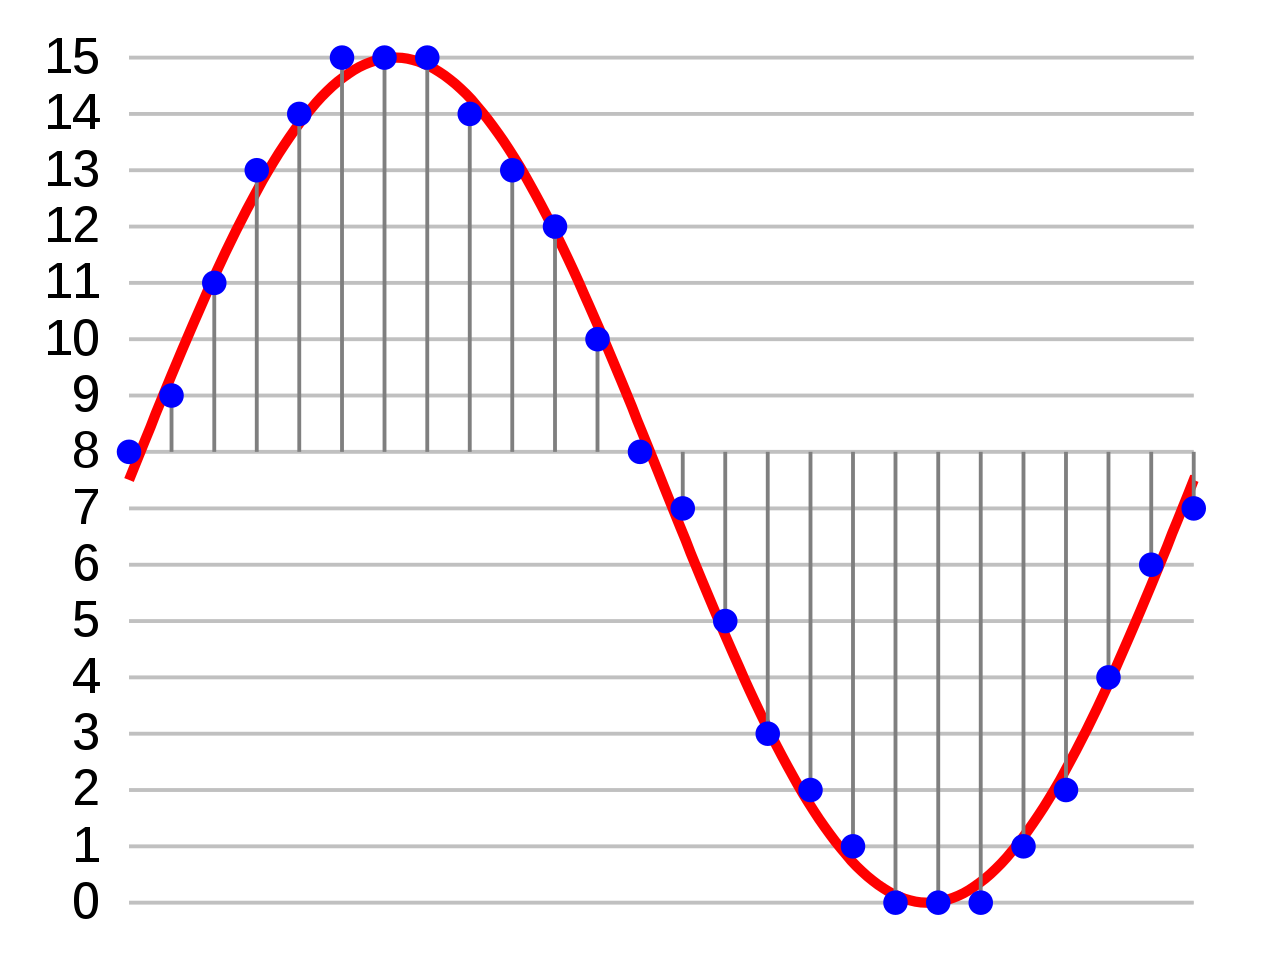
\includegraphics[width=0.5\textwidth]{pcm.png}
		\caption{Linear pulse-code modulation at 4 bit depth.}
		\label{fig:pcm}
	\end{figure}
	The method that makes sampling a possibility is Pulse-Code Modulation (PCM for short). Dating back to the 1930s, it consists of the digital representation of analog signals, and is subject to two parameters: sampling rate and bit depth. This technique processes an input analog signal by making readings of voltage levels at fixed time intervals and transforming them into numeric values. Commonly referred to as samples, these readings are what the resulting digital representation will be composed of. The sampling rate refers to how often samples will be read from the analog signal, and the bit depth indicates the amount of bits with dedicated to the storage of each sample. Every time an analog reading is being converted into a digital sample, it is rounded to the nearest integer value in the range determined by the bit depth. This rounding process, visible in Figure \ref{fig:pcm} \cite{pcm_img} is known as quantization. Since samples are encoded to integers in binary, the levels to which they can be quantized are uniformly distributed. This describes the method of Linear PCM (LPCM), a sub-method of PCM that is used for audio CDs and the popular formats WAVE and AIFF, among other applications.\par
	

	
	\subsubsection{Modern music production} 	
 	In a world of highly complex information systems, digital music production has been developed thoroughly. When it comes to modern music composition, Musical Instrument Digital Interface (MIDI from now on) % TODO cita
 	protocol provides grounds for an alternative to regular, "analog" instruments. This standard erects a bridge for communication between digital instruments and computers, providing the world of digital music production with the tangible interfaces of normal instruments. The MIDI standard provides, among many other features, a communications protocol that encodes music events. This manifests in the form of messages which describe data such as the pressing, releasing, and velocity of musical notes. 	
	 	
 	A digital audio workstation (DAW from here on out) is a software environment for music production. These workstations revolve around MIDI, which provides an encoded language for musical notes. See Table \ref{table:notes} for a table of the syllabic and alphabetical equivalents of musical notes. Note-related MIDI messages always store data regarding the note subject to the event. 
 	\par
	\begin{table}[h] % TODO add MIDI code column
		\centering
		\begin{tabular}{c c}
			Syllabic & Alphabetical \tabularnewline
			\midrule
			Do  & C \tabularnewline
			Re  & D \tabularnewline
			Mi  & E \tabularnewline
			Fa  & F \tabularnewline
			Sol & G \tabularnewline
			La  & A \tabularnewline
			Si  & B \tabularnewline
		\end{tabular}
		\caption{Musical notes in syllabic and alphabetical form}
		\label{table:notes}
	\end{table} 
	One can have an extensive range of digital synthesizers, samplers, and effect chains all working simultaneously in a DAW, the type of software that provides a playground that routes audio between racks of components and effects, making music production a possibility to anyone that owns a computer. DAWs have an element known as a \textit{piano roll}, which serves as a sort of digital equivalent to sheet music. The piano roll is where producers draw out musical events, placing small rectangles on a grid to represent the notes, their length, and their duration. % TODO image proll
	The arrangements of events are then encapsulated in what are called patterns. These patterns can be applied to instruments, such as synthesizers, or samplers, to trigger the sounds they produce. Patterns can be drawn out manually, auto generated, or recorded in real time with a MIDI controller. Auto generated patterns may consist in filling a set length of time with notes separated by constant intervals, so as to mimic the timing of a metronome, for example. Patterns that are recorded in real time are made with the DAWs recording function, which is activated to record MIDI events from a controller. \par 

	When recording patterns, incoming MIDI events are timestamped to then be displayed in chronological order and resemble the translation of the user's input. A user may have an instrument loaded during this recording period, so the user can hear what sounds are being produced. It is important to highlight what is captured by the DAW is a sequence of MIDI events, not the actual sounds being produced by the instrument, meaning that a pattern is just a sequence of data, void of sound until an instrument that can process the events is associated to it. More so, since patterns are composed of MIDI events meant to trigger responses from instruments, there is no binding between them and instruments, and a pattern made for one instrument can perfectly be used for another. \par 
	
	The most relevant events associated to the pattern building process are: note-on events, the signal that a note has been pressed; note-off events, the signal that a note has been released. The subtraction of the timestamps associated to these two events determines how long a note is held down. A musical note is associated to note-on and note-off events, having the note and octave being encoded as an integer in the range of $[0, 128)$. In addition, associated to note-on events is an element called velocity, which is a measure of the intensity of the note. The velocity of a note is sometimes processed by instruments to generate softer or stronger sounds. Some samplers use note velocity to trigger a sample from a set, i.e. a lower intensity recording of a snare drum for lower velocities as opposed to a sample of a powerful snare drum hit when the velocity is a higher range.
 	\par
 	
	DAWs can be extended with plugins in the form of effects or instruments. The former normally have a sound-based input-output relation with the DAW, meanwhile instruments will take MIDI messages and produce a sound as an output. The most common standard for plugins is Virtual Studio Technology (VST), created by a german company called Steinberg. VST plugins have multi platform support on major operating systems, however, plugins must be exported for a target operating system, i.e. a VST plugin that is exported for Windows will not work on Mac OS or Linux. A possible VST plugin could be a sine wave based instrument, for example. The wave's frequency will depend on the key being pressed, and the force applied to the key will dictate the amplitude of the wave. This plugin, although simple, could be considered a synthesizer. \par 
	A sampler is a synthesizer that uses samples rather than oscillators to produce sound.  The sources of the sounds it produces are samples, which can be described as clips of audio that are stored in a digital format within the sampler's memory. You're likely to find that hardware and software samplers offer sets of "stock" samples that are loaded by default. The option to load samples from an external source such as an SD card is also common, just like recording external input from a recording device such as a microphone. As is the case with non sample based synthesizers, there are a variety of ways that samples can be manipulated in order to tweak the produced sound to the user's liking\par
	
	\subsubsection{Sampling technique} \label{st}
	The key concept of sampling techniques is to modify and manipulate audio samples to create sounds. Many types of transformations can be applied to samples in order to drastically change the way they sound, although products that sound far different to the source sample are not always the objective. A sample can be manipulated by delimiting subsections within it, so as to create separated sub-samples that can be treated as individual notes. This process is colloquially referred to as \textit{chopping} the sample, resulting in a set of \textit{chops}, the sub-samples obtained from the main sample. \par
	Another way to manipulate a sample is via \textit{envelopes}, which dictate the way a sound changes over time. Envelopes affect playback every time it is triggered, and are commonly composed of four parameters. The first one  comes into play upon note-on events, i.e. on a key press: \textit{attack}, describing the time it takes for the sound's level to rise from zero to its peak. Next, \textit{sustain} is the level at which the sound will hold until a note-off event, i.e. when a key is released. \textit{Decay} depends on sustain, and it describes the time it will take for the level to go from peak to sustain. Finally, \textit{release} is the tail end of the envelope. Starting on note-off events, it describes the time it will take to reach zero level from sustain level. These four concepts form the acronym ADSR, and can be pictured as a plot of level against time in Figure \ref{fig:envelope}. You may have noticed that three of the parameters refer to a time measure, whereas sustain refers to a level. \par
	
	
	\begin{figure}[h]
		\centering
		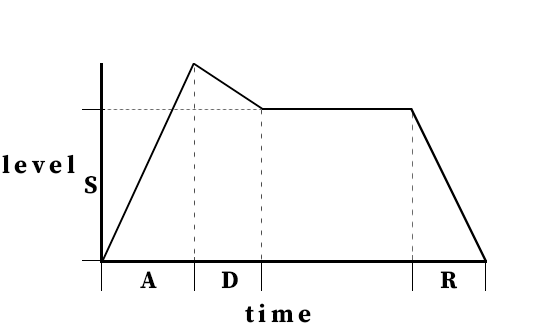
\includegraphics[scale=0.4]{envelope.png}
		\caption{ADSR parameters in envelopes}
		\label{fig:envelope}
	\end{figure}
	
 	The entity that is the sample based instrument is what holds and modifies the configuration that revolves around a main sample. It knows where to find the main sample, where each subsection starts and ends, and what the envelope parameters are set to for each chop. The sampler is equipped for playback, and is configurable in the way sounds interact as they are triggered. \par 
 	A parameter that can be found in most instruments is termed \textit{polyphony}, a measure that limits the playback at any moment to a particular number of sounds. Polyphony is commonly described with an arbitrary number of \textit{voices}. An instrument with 3 voices can play at most 3 sounds at any point in time, for example.\par
 	Furthermore, a series of effects may be applied to the sample in order to modify the sound that is output. Filters and compressors are some of the most common effects you may come across. Filters eliminate frequencies from the sound. Compressors apply reduction to the sound when the level crosses a certain threshold. Being applicable to any source of sound, these types of effects are most likely included with any arbitrary DAW, although they are sometimes also found within samplers.

	
	\newpage
	\subsection{Motivation}
	Modern DAWs have built in samplers or similar tools that allow a user to sample sound and directly manipulate it so as to employ sampling techniques. In most cases, these tools are more than capable of providing the means to translate these techniques into action, however, depending on the DAW, you may be hindered due to the workstation's design. Whether it be the user interface, the imposed workflow, or the minimum amount of steps required to reach your sampling goals, I have found that the process is likely to involve obtrusive inconveniences.\par
	 
	Personally, I find that there are a minimum of three steps to achieve a usable sampler configuration. First, a main sample must be loaded. Second, a number of chops are delimited in the bounds of the main sample. Third comes the assignment of chops to MIDI notes, in other words, the mapping of sample subsection playback to a controller's keys. These steps are a prerequisite to playing chops on a controller, or to lay notes out within the DAW's sequencer. At this stage, the user can experience the instrument and judge whether it is necessary to take a step back and make adjustments, for example, shifting the start time of a chop, creating/deleting a chop, or moving the trigger note to another of higher convenience. All of this implies that the design of a sampler instrument is an iterative process, and that the user may keep reforming it in several ways to fit the necessities of the creative process in musical composition. \par 
	
	Since the essential number of steps and functions required to obtain a usable instrument are few, there is room for improvement in comparison to the process that takes place when using the tools inherently available in an arbitrary DAW. By focusing on the indispensable functions and actions, the process can be simplified to provide a fast way of putting together a sample based instrument. Hindrances such as overloaded user interfaces are eliminated, leaving out the buttons and functionalities that are seldom used and may cause distractions on the creative process. \par
	
	By implementing the instrument as a VST plugin, a vast number of DAWs become candidates for the inclusion of this plugin and a streamlined sampling process. Any DAW's inherent limitations and/or hindrances would no longer be obstacles when it comes to creating a sample based instrument. This way, an instrument strictly designed for sampling would be attachable to a large number of workstations, providing a simple way to put sampling techniques to use on most platforms.
	  

	
	
	\newpage
	\subsection{Objectives}

	For the simple implications of sampling techniques, the means by which you achieve a minimum setup with which you can play around and manifest ideas should be straightforward. The aim is to reduce the amount of user interaction required to reach a usable sample based instrument. To do so, I will downsize in the features that any arbitrary DAW has to offer, including only those that are strictly necessary. This translates to the reduction of hindrances that may arise when there is an excess amount of functionality that is rarely used.  By implementing the instrument as a VST plugin, I aspire to build an accessible sample based instrument optimized for the application  of sampling techniques. %This means that the user will be able to load, chop, and play samples with speed and ease in a reduced sequence of actions. In addition, the user should also be able to make fast corrections and tweaks to further develop the instrument. 
	\par
	The core capabilities the sampler can be listed as four points:
	\begin{itemize}
		\item Providing a visual representation and an audio preview of the main 
		sample and its chops.
		\item A way to create subsections in the audio clip.
		\item List component that shows all chops and the trigger notes they are associated to.
		\item The ability to play individual chops in response to triggering MIDI events.
	\end{itemize}
	
	Furthermore, there are more features that would be of great value, such as the following:
	\begin{itemize}
		\item \textit{Automatic} chop creation using peak detection algorithms.
		\item Chop playback: adjustable envelope parameters for each chop, and a polyphony setting for the sampler as a whole.
		\item The ability to load and manage a set of main audio samples simultaneously.
		\item Plugin state saving and loading, for the storage and recovery of configurations.
		\item Pitch shifting algorithms to modify the tone of the main sample and its chops.
		\item A series of effects for each chop: filters, compressors, 
	\end{itemize}

		\newpage	
	\section{Plugin design}

	This section will provide an overview of the the usage and configuration of the instrument in an audio workstation. In this guide, the DAW that will host the plugin is Reaper \cite{reaper} on a computer running Windows. This feature rich software can be evaluated for free, and has support for VST plugins. Download \cite{plugin} and place the plugin in the C:$\backslash$Program Files$\backslash$Common Files$\backslash$VST3 directory.
	As additional preparation for the process, it is useful to have an audio file of WAVE format ready, as well as a MIDI controller connected to the machine.\par
	
	To begin, open Reaper and open the \textit{Preferences} dialog under the \textit{Options} menu. In the list of categories on the left, select the \textit{MIDI Devices} (figure \ref{fig:udevoff}) option under the \textit{Audio} section. 
	\begin{figure}[h]
		\centering
		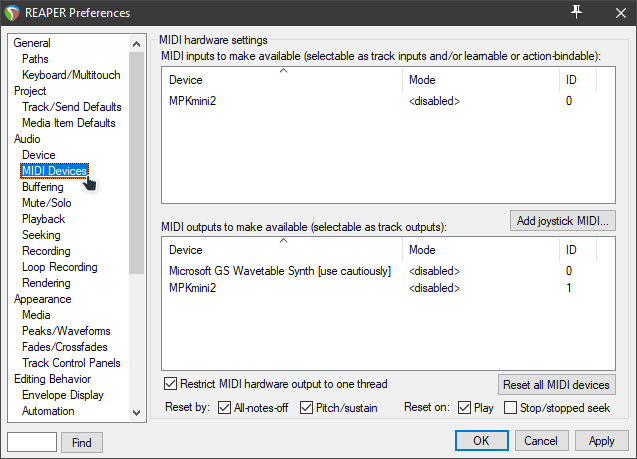
\includegraphics[width=0.7\textwidth]{u/dev_off.png}
		\caption{MIDI devices preferences.}
		\label{fig:udevoff}
	\end{figure}
	
	Your MIDI controller should appear in the upper box of MIDI inputs. Right click on the device and enable it if is disabled as shown in figure \ref{fig:udevon}.
	\begin{figure}[h]
		\centering
		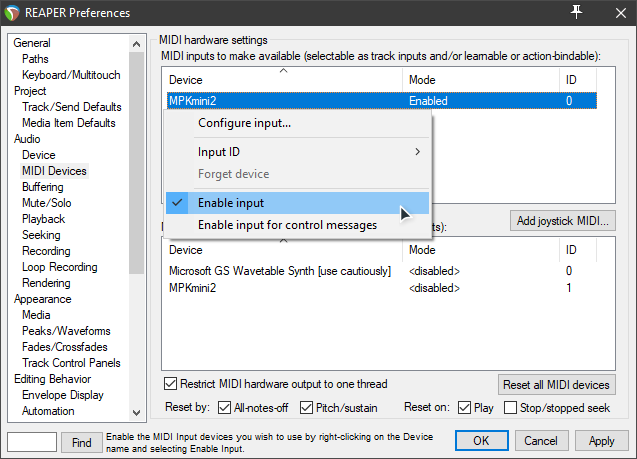
\includegraphics[width=0.7\textwidth]{u/dev_on.png}
		\caption{An enabled MIDI controller.}
		\label{fig:udevon}
	\end{figure}
	
	Next, add an instrument track from the \textit{Insert} menu, with the \textit{Virtual instrument on new track...} option. On the window that pops up, you can type JCS in the filter field on the bottom. The plugin should appear as shown on figure \ref{fig:load}. If it isn't shown, make sure Sampler.vst3 exists in the directory C:$\backslash$Program Files$\backslash$Common Files$\backslash$VST3 and refresh the list under \textit{FX} $\rightarrow$ \textit{Scan for new plugins}. Press OK to load the sampler onto the instrument track, and a new window will pop up with the a blank plugin.
	
	\begin{figure}[h]
		\centering
		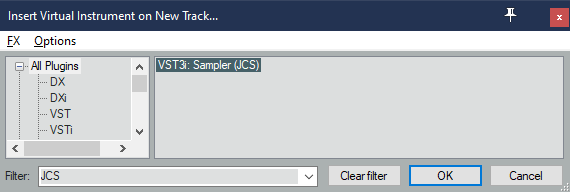
\includegraphics[width=0.9\textwidth]{u/load.png}
		\caption{Selecting the plugin in the virtual instrument dialog.}
		\label{fig:load}
	\end{figure}
	
	~\\
	~\\
	Start by loading a WAVE file as the main audio sample with the \textit{Load} button on the top left corner. The waveform representation of the file will be visible in the thumbnail. The slider to the right of the thumbnail is a control of the thumbnail's scale, while the slider beneath is for horizontal scrolling when the scale is larger than the thumbnail's boundaries. The preview's playback can be controlled with the \textit{Play}, \textit{Pause}, and \textit{Stop} buttons on the panel to the left. \par 
	The bar located above the thumbnail holds a \textit{Position} label, which indicates the position of the playback head for the audio preview. This position is also relevant for the manual creation of subsections. Playback can be looped in the full boundaries of the audio file with the \textit{Toggle Full Loop} button. The playback position can be manually positioned by clicking on any part of the thumbnail, and a selection can be made if a click is dragged across the desired area. After making a selection, you can loop the audio preview within the selection's boundaries with the \textit{Toggle Loop Selection} button. \par
	
	Chop creation can happen in two different ways:
	\paragraph{Manual chopping\\}
	The two buttons located above the thumbnail on the top right corner of the plugin create chops. The first, \textit{Chop From Here} will use the region between the current position and the end of the sample to create a chop. The second option will only be available if a selection is exists in the thumbnail, and it will create a chop with boundaries equal to those of the selection.
	\paragraph{Automatic chopping\\}
	If your audio clip has noticeable peaks, where the level of sound changes notably and within a short time frame, then automatic chopping provides a fast way to split the sample into regions separated by sharp peaks. The \textit{Chop} button will create as many chops as chops are detected. This number will differ depending on the configurations of the mode and threshold, which can be modified with the button and slider. The changes made to these two options will be reflected in the label placed under them, which indicates how many chops are detected with the current configuration.\par
	
	\begin{figure}[h!]
		\centering
		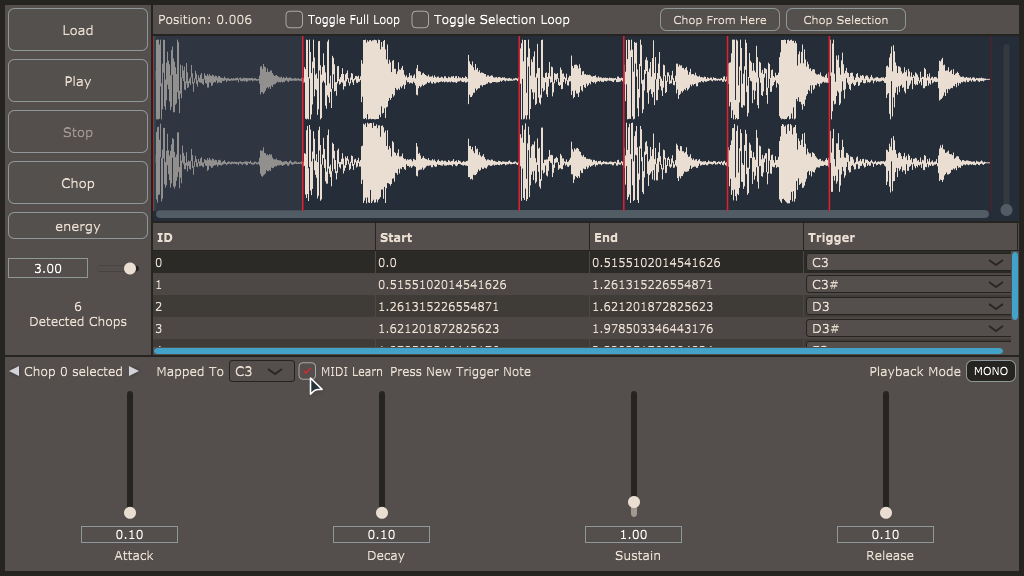
\includegraphics[width=0.9\textwidth]{u/learn.png}
		\caption{Reassigning trigger notes with MIDI Learn.}
		\label{fig:learn}
	\end{figure}	
	
	~\\
	After chopping the sample, the table under the thumbnail will display the details for each chop. Trigger notes can be changed from the last column in the table, or they can be changed by pressing a note on your controller with the MIDI Learn function. To do this, select a chop from the table by clicking on it and press the MIDI Learn button located under the table. As shown in figure \ref{fig:learn}, a label that reads \textit{Press New Trigger Note} will be displayed, and the trigger note will be updated to the next note you press on the controller. \par
	
	A chop can be selected for further editing with a simple left click on a row from the table, or you can scroll through the chops with the arrows on the top left part of the lowest panel. The selected chop's playback can be tweaked with the envelope parameters in this lower panel. Each parameter will affect the way the chop sounds over time. The purpose of each parameter is explained in section \ref{st}. The instrument's polyphony can be changed in this panel as well: to allow for more than one chop to sound at the same time, change the \textit{Playback Mode} on the top right part of the lower panel to POLY. When set to MONO, chops are played exclusively, and the triggering of one chop will cut off the playback of any other.
	
	The instrument is now playable, and a series of notes can be sequenced in Reaper. You can try out different combinations of notes to see the order in which they sound best to you. To record your sequence, press the red \textit{Record} button visible in figure \ref{fig:rec}. When recording, Reaper will save the MIDI notes you press into a MIDI item, which can be found in the playlist to the right of the instrument rack. \par
	
	
	\begin{figure}[h!]
		\centering
		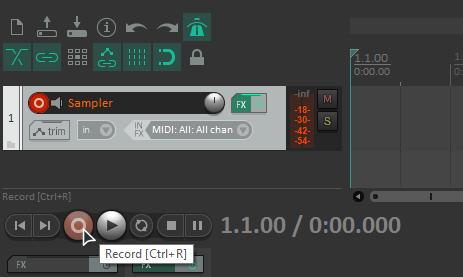
\includegraphics[width=0.9\textwidth]{u/rec.png}
		\caption{Record button in Reaper.}
		\label{fig:rec}
	\end{figure}
	
	\newpage
	\section{Implementation}
	\subsection{Technologies}	
	\paragraph{JUCE framework\\}
	%intro juce, support for plugins, extensive tutorials and examples
	To implement the sampler, I used an application framework called JUCE\cite{juceweb}. It has cross-platform support and is written in C++. It is the best choice because  it is a mature project that is still growing, and I am familiar and comfortable with C++. It is also open-source and licensed for free for personal, non-commercial use. The amount of documentation and tutorials available online was enough to convince me that I would need nothing else to implement the majority of the instrument.
	
	% how does juce work? what does it offer? object oriented, event driven 
	JUCE makes use of the object oriented capabilities of C++ to present a wide array of classes and utilities. It offers the building blocks to application development with a reasonably gentle learning curve that discards the need to reinvent the wheel. These utilities help with tasks that range from audio playback, to event driven data structures, to the design of user interfaces. Furthermore, the framework is in line with the event-driven paradigm, which makes the development of action based applications a simple and efficient task. As stated, the documentation is vast and there are numerous descriptive tutorials. On top of that, at the programmers disposal are more than 70 example applications that showcase the several features the framework has to offer. 
	
	\paragraph{Projucer\\}
	The Projucer is JUCE's cross-platform application that allows for the creation, management and configuration of JUCE projects. To enable development on Linux, for example, one can add a Makefile exporter to their project. The Projucer will create an architecture specific Makefile that links external libraries and builds the application. The templates offered from which to start new projects include GUI Application, Animated Application, Console Application, Audio Application, Audio Plugin, and Static Library and Dynamic Library. Each of these archetypes are configurable in distinct ways, and are initialized to include the fundamental code inherent to the nature of the application. For Audio Plugin projects, the Projucer can export several plugin formats, such that one build process compiles and exports the plugin formats that the project is configured to build. The formats include VST and Standalone Application, among other less relevant plugin formats. Building a Standalone Application allows for the usage of the plugin without the need of a DAW. Building VST plugins is only supported on Windows, which means that for development on Linux, one can only test the build in an isolated, standalone application, void of connections to a DAW. \par
	
	% 0. explain components and structure of project
	The Projucer's base audio plugin project provides fundamental code containing two classes. The dichotomy encourages the separation of the audio processing logic from the GUI side of the plugin. The \textit{PluginProcessor}, as the name suggests, is the audio processing heart of the application. This class extends the \textit{AudioProcessor} class, a base class for audio processing. This is where tasks such as MIDI connection management and audio rendering take place. In addition, this class holds the data model of the current configuration as the plugin's state, used to construct the the visual representation of the plugin, which is rebuilt every time it is restored from a minimized state.\par
	The \textit{PluginEditor} extends from the \textit{AudioProcessorEditor} class. It is the object that builds the user interface and responds to interaction with graphical elements. Unlike the \textit{AudioProcessor} class, which inherits from no other, the \textit{AudioProcessorEditor} class extends from the \textit{Component} class. This is the base class for a wide range of user interface objects. The \textit{Component} class has two virtual functions that are to be overridden by any class derived from it: \texttt{paint()}, the function that dictates the on screen layout of the component; \texttt{resized()}, which contains reactionary logic for when the component is resized. Both functions are callbacks, which means they are invoked automatically upon triggering events.\par 
	
	
	\paragraph{Aubio\\}
	The aubio library is a set of tools designed for the extraction of annotations from audio signals\cite{aubio}. Being an open source library written in C, it seemed a perfectly suitable inclusion to the sampler. One of the modules included with the library serves as a detector of peaks in audio files. Sample chopping is regularly done at the beginning of notably strong sonic impacts, such as drum sounds. The library enables the automatic chopping process for these cases, when the user wants the subsection delimiters to be placed exactly before peaks, so this is a feature that would be of great benefit to the plugin.
	
	\paragraph{Alternatives\\}
	For the automatic creation of audio regions, the vamp\cite{vamp} library could have been a viable alternative to aubio\cite{aubio}. It provides an onset detection module\cite{vamponset} and uses C/C++ interfaces, so it has equal offerings to aubio, essentially. After trying aubio's onset detection module and successfully integrating it within the plugin, I decided to keep it and forgo vamp, as aubio had a variety of different detection methods which seems to be sufficient for the purpose of automatic sample splitting.\par	
	Another possible implementation could have been based on jVSTwRapper\cite{jVSTwRapper}. This library is based on Java for development of VST audio plugins. It is open source, which makes it suitable for the task at hand, and based on a language I am also comfortable using. It is a smaller and younger project, bringing up inconveniences such as the lack of features and abundance in comparison to JUCE. 
	
	
	\newpage	
	\subsection{Audio preview}	
	The first step in developing the sampler consisted in loading an audio file. With the help of the \textit{Draw audio waveforms} tutorial \cite{audiothumbnail}, I was quickly able to identify the classes I would need to load, and, additionally, display a visual representation of an audio file. For starts, a \textit{FileChooser} object is used to create a dialog box that selects files or folders. One can limit the formats allowed for selection by specifying semicolon separated regular expressions in its constructor. Using the string \texttt{"*.wav"} as the \texttt{filePatternsAllowed} parameter will only allow users to select WAVE files, for example. The class offers several member functions named with "\texttt{browseFor}" as a prefix, and \texttt{browseForFileToOpen()} opens a dialog box to select a file for opening, returning a boolean value that indicates whether the user selected a file or not. In the former case, the FileChooser's \texttt{getResult()} function will return the \textit{File} object that was selected. \par
	The class that would provide the visual representation of the audio file is the \textit{AudioThumbnail} class. It works hand in hand with the \textit{AudioThumbnailCache} class, which serves as a cache memory of audio file representations. Together, they store and print waveform representations of audio files. I created a separate class \textit{SamplerThumbnail} to bundle the \textit{AudioThumbnail} object and its related objects and functions into a separate component. For the thumbnail view to load the audio file, I created a public function \texttt{setFile(const File\& file)} within the \textit{SamplerThumbnail} class. Within \texttt{setFile}, the audio file is loaded with the \texttt{setSource(FileInputSource* newSource)} function of \textit{AudioThumbnail}. The \textit{FileInputSource} object can be created from the \textit{File} received from the \textit{PluginEditor} by passing the file as the only parameter to the constructor of a \textit{FileInputSource} object. With this done, the \textit{AudioThumbnail} will load the waveform representation of user-selected audio files.\par
	

	% PLAYBACK
	Audio playback is achieved through the \textit{AudioTransportSource} class, which enables the audio preview of the main sample that is loaded in the plugin. It inherits from the \textit{AudioSource} class, which is a base class that enables continuous audio playback. The \textit{AudioTransportSource} is used because it implements can be positioned, played, paused, and stopped. These features are useful for previewing the initially loaded sample. Audio subsection playback is handled differently, and will be discussed later on. The connection of audio files to the \textit{AudioTransportSource} object is achieved via \textit{AudioSource} subclasses. In this case, an \textit{AudioFormatReaderSource}. The processor stores an instance of \textit{AudioFormatReaderSource} in \texttt{currentAudioFileSource}, and in \texttt{transportSource} an instance of \textit{AudioTransportSource}. \textit{AudioFormatReaderSource} objects of this class obtain streams of sound from \textit{AudioFormatReader} objects, which source their sound from audio file streams. Every time a user opens a file successfully, a function \texttt{loadFileIntoTransport(const File\& file)} is executed. This function will stop the \textit{AudioTransportSource} from continuing playback, and proceed to change the source. To do this, a new \textit{AudioFormatReader} object is created for \texttt{file}. This is done through an \texttt{AudioFormatManager} object, which is used to keep a list of the formats that are to be accepted by the application. It includes a method called \texttt{AudioFormatReader* createReaderFor (const File\& file)}, which returns a pointer to the \textit{AudioFormatReader} that is necessary for the creation of an \textit{AudioFormatReaderSource}. If \texttt{createReaderFor} fails, it returns a null pointer, so the following steps are only taken in cases where the pointer is not null. The \texttt{currentAudioFileSource} pointer is reset to the new reader source, and the \texttt{transportSource}'s new source is set with \texttt{setSource}.\\
	All of these instances and connections lead to a functional way to play audio, however, there still is the need to connect the \texttt{transportSource}'s interface to GUI elements. The \textit{AudioTransportSource} class extends \textit{ChangeBroadcaster}, which allows for event driven reactivity to the state of the \textit{transportSource} object. To aid in the process, an \texttt{enum TransportState} is declared to include the states of \texttt{Stopping}, \texttt{Stopped}, \texttt{Starting}, \texttt{Playing}, \texttt{Pausing}, and \texttt{Paused}. Buttons layed out in the application will change a private variable \texttt{TransportState state} to \texttt{Starting}, \texttt{Stopping}, and \texttt{Pausing} to invoke \texttt{transportSource.start()} or \texttt{transportSource.stop()}. By executing these methods of the \texttt{transportSource}, every object that extends \textit{ChangeListener} that has been added to the \texttt{transportSource}'s list of listeners will be notified of a change. This notification manifests by invoking the callback function \texttt{void changeListenerCallback (ChangeBroadcaster*\\ source)}, which is a virtual function that must be implemented by any class that extends \textit{ChangeListener}. The plugin editor extends this class and adds itself to the \texttt{transportSource}'s listener list with the following instruction: \texttt{transportSource.addChangeListener(this);}. In the \texttt{changeListener-\\
	Callback} function, the source of the event is checked by comparing references like so:
	\begin{verbatim}
	void changeListenerCallback (ChangeBroadcaster* source) override
	{
	if (source == &transportSource)
	{...
	\end{verbatim}
	Inside the conditional block, the transport state is updated once more, and the GUI is synchronized in accordance to the next transport state, for example, when \texttt{Starting}, the state transitions to \texttt{Playing}, changing the play button's text to "Pause" and enabling the stop button. \par
	
	
	\newpage
	\subsection{Chopping the main sample}
	Chops are modelled as a struct and are comprised of 6 fields: an unique identifier, start and stop times and samples, the trigger note, and a boolean value named \textit{hidden}. Start and stop measures are stored in seconds and samples. The trigger note is an integer encoding the MIDI note that is associated to the chop, and the \textit{hidden} field dictates the chops' visibility in the components that display chops. \par 
	The storage of these fields is done via the \textit{ValueTree}\cite{valuetree} class, which is a lightweight data structure that is capable of handling datatypes of all sorts, storing a list of properties, subtrees, and references to shared data containers. Using a struct to wrap this data structure brings the benefit of type and validity checks when creating chops. The creation of a chop with this construct creates a \textit{ValueTree} object, setting the values for properties that resemble the fields previously described after performing some checks. This \textit{ValueTree} can then be added to the general \textit{ValueTree} that stores all chops with an assurance of validity in terms of types and value boundaries. The \textit{ValueTree} data structure supports event-driven programming: listeners can subscribe to a tree in order to invoke callbacks when events arise, such as property changes or the removal/addition of a subtree.
	
	
	\subsubsection{Manual creation}
	The \textit{AudioThumbnail} component plays a big part in manual chop creation. Since it displays a visual representation of the sample, it is possible to recognize patterns in the waveform to estimate the position and length of the subsection you wish to create. By default, the \textit{AudioThumbnail} does not interface with mouse clicks. Nevertheless, the interception of clicks as events with coordinates is fully supported. I found out about this through the \textit{AudioPlaybackDemo} that is part of the Projucer's examples, where it was possible to click on the \textit{AudioThumbnail} to relocate the playback head of the \textit{AudioTransportSource} to any position on the waveform.\par
	 
	To do this, the \textit{AudioThumbnail} is instantiated as a member and placed within a parent component. This way, the parent component can override functions such as \texttt{void mouseDown (const MouseEvent\& e)} and \texttt{void mouseDrag (const MouseEvent\& e)} to define the interactions between the component and events triggered by the mouse. When one clicks on the thumbnail, the coordinates of the click event are part of the event's payload. The \textit{x} coordinate is all that is needed to obtain the equivalent point in time in the sample: it is done with a few arithmetic operations that use the parent component's and the thumbnail's width and the as operands, as well as the \textit{x} coordinate. This works both ways, such that a position in time can be converted to an \textit{x} coordinate. This feature allows for the rendering of a playback head that scrolls along the thumbnail as it plays in real time. Likewise, when a chop is created, its boundaries can be drawn upon the thumbnail with two markers to indicate the region it is contained in.\par
	
	The thumbnail then becomes the means through which manual chop creation is possible. One way of creating a subsection is goes by the name of \textit{Chop selection}. This is based on the possibility of overriding the \texttt{mouseDrag} function to display rectangles resembling selections over the thumbnail. The coordinates of the limits of these selected areas are stored upon the firing of the drag event. These pairs of coordinates are used to draw a see-through rectangles over the thumbnail, and, if need be, to create a chop out of the boundaries of the selection. Termed \textit{Chop from here} is the second way to manually create chops. On activation, this option uses only the earliest coordinate of the thumbnail selection, making chop's end point always coincide with the end of the main sample. \par

	\subsubsection{Peak detection}
	Automatic chopping is achieved through the aubio library. To interface with the library from the application, the Projucer must know the paths to the libraries and the header files. It then adjusts the exporter in order to link the libraries when building the application.\par	
	Onset, meaning the start of a musical note, is the name of the module relevant to this task. To use the peak or onset detection algorithms provided by aubio, the first step is to create a source object to be later passed onto the onset object. The source is created using the path to the file and the sample rate of the file. These values are found through two members of the \textit{PluginProcessor} class, with the \textit{File} object's  \texttt{getFullPathName()} function and the \textit{AudioFormatReaderSource} object's \texttt{getAudioFormatReader()->sampleRate} attribute. \par
	
	The library provides a range of eight different onset detection methods, so I created a button that allows for the selection of any method. To indicate the detection sensibility, the onset object requires a threshold be set, via\\
	\texttt{aubio\_onset\_set\_threshold(aubio\_onset\_t * o, smpl\_t threshold)}.\\
	The desired threshold is selectable with a slider element in the user interface. The plugin editor registers as a listener to this slider to know when the value of the threshold is changed. This is done to provide an anticipation of the number of chops that would be created with any configuration of an onset method and an arbitrary threshold setting. \par
	
	Finally, associated to the press of a button, the execution of the onset algorithm is triggered with the current threshold value and onset method. Chops are created in the non-overlapping areas delimited by the detected peaks. In other words, the first chop begins on the first peak and ends on the second peak, the second begins on the second peak and ends on the third peak, etc.
	
	
	\subsection{Subsection management}
    A table component was included to visualize the amount of chops and some of their details. Initially empty, the table sees the addition of rows as chops are created. Rows are composed of four fields of information related to the chop: one for the chop's unique identifier, another two dedicated to the start and stop times describing the region covered by the chop, and a final one for the note that triggers the chop's playback.
    The latter field is interactive in the sense that it is represented with a drop down list, allowing the reassigning of chops' trigger notes. The notion of the essential steps to implement \textit{custom} cells for the trigger note column was easily captured with the help of the table list box tutorial\cite{tablelistbox}. Furthermore, I added right click interaction with rows to open a menu from which chops can be deleted and hidden.\par %IFNEEDED popupmenu connection
    
	The chop list table allows for the selection of single rows. The selection of a row triggers a change on the thumbnail, which highlights the region associated to the chop. To do so, the chop list component keeps a member variable of the \textit{Value} class named \texttt{selectedChop}. The \textit{Value} class is a wrapper around a shared, reference-counted underlying data object \cite{value}. It allows for the notification of changes to attached listeners, which is the main reason for choosing the \textit{Value} class for this variable. Whenever the table's selected row changes, the thumbnail and other listening components will execute callback functions to react to the changes immediately. \par
	
	On the lower part of the user interface is the chop settings component. By registering as a listener to the chop list component's \texttt{selectedChop} variable, this panel displays the selected chop's envelope parameters, which can be modified in order to determine the behavior of its playback over time. Each envelope parameter is associated to a \textit{LabelledSlider} object, a component with the necessary objects that are a common factor to all parameters: a slider for its value and a label for its name. As will be mentioned in detail later on, each chop is associated to a \textit{SamplerSound} object, which is responsible for it's playback. This object is the place to set the envelope parameters for each chop, so it is necessary to modify these whenever a parameter is changed. \par
	
	Another function included in the chop settings component allows for the definition of the instrument's polyphony. With a button that toggles between modes, the two settings are termed \textit{mono} and \textit{poly}. On one hand, \textit{mono} playback will give the instrument one single voice for sound playback. One voice can play at most one sound, and, as stated in the previous paragraph, each chop is assigned a \textit{SamplerSound} object for playback. This means that \textit{mono} mode will only permit at most one chop to sound at any given moment: if a chop's playback is triggered while another is being played, the most recently activated chop will begin playback and cut off the previous. On the other hand, \textit{poly} playback will create one voice per chop, allowing that every chop be played at the same time. Just like with the \texttt{selectedChop} variable, the chop settings component holds an instance of the \textit{Value} class named \texttt{playbackMode}. The \textit{SamplerAudioSource} component, in charge of managing sounds and voices, among other tasks, registers as a listener to \texttt{playbackMode} to reset the number of voices in accordance with the newest value for the instrument's polyphony setting.\par
	
	For a more tangible and straightforward way to reassign chops' trigger notes, the chop settings section includes the concept colloquially known as MIDI Learn. It achieves the task of rebinding the note by \textit{listening} to the connected MIDI controller. When a MIDI note press event is detected, the chop's trigger note is assigned to the event's note. This feature also makes use of the \textit{Value} class.  The processor declares one to know what the last recorded MIDI note is, and the chop settings component declares another to dictate whether or not to listen to MIDI notes at all. The latter, named \texttt{listenForMidiLearn} is listened to by the processor in order to dictate whether or not to update the former \textit{Value} \texttt{lastRecordedMidiNote} to that of the incoming MIDI notes. The chop settings component listens to \texttt{lastRecordedMidiNote} to finally update the chop's trigger note with the note newly detected by the processor. In doing so, the chop list component notifies the processor via \texttt{listenForMidiLearn} that \texttt{lastRecordedMidiNote} should no longer updated.
	
	
	
	\newpage
	\subsection{Audio playback}
	The object in charge of translating trigger notes to production of sound in this instrument is the \textit{SamplerAudioSource}. This class extends the \textit{AudioSource} class, meaning that it is equipped for continuous audio playback, just like the aforementioned \textit{AudioTransportSource}. With the addition of this audio source for the playback of individual chops, the plugin now has two audio outputs (since the transport source is still present for the audio preview of the main sample). To support both of these sources, the \textit{MixerAudioSource} presents a simple solution. Like both sources, this class also extends the \textit{AudioSource} class, and it mixes the output of several audio sources into one, making the mixer source the desired audio source for the plugin's output signal. Both audio sources are connected to the mixer, which is set as an \textit{AudioSourcePlayer} object's source, which accepts a single audio source as input. This chain ends with the source player, which is what enables continuous audio playback from an audio source. Now for the ways sound is created in the sampler audio source. \par
	
	An object of the \textit{Synthesizer} class is held within the \textit{SamplerAudioSource} class, where the connection is made between sounds and voices and the synthesizer. As mentioned in previously, the playback of chops happens through objects termed sounds. These objects extend the \textit{SynthesizerSound} class and are sounds that a synthesizer can play. Likewise, \textit{SynthesizerVoice} objects are the voices that a synthesizer is equipped with to play instances of the \textit{SynthesizerSound} class. The \textit{SamplerSound} and \textit{SamplerVoice} classes are the sound and voice implementations chosen for the synthesizer, due to their ability to source sound from audio files. \textit{SamplerSound} objects are constructed with an object of the class \textit{AudioFormatReader} that represents the file to source the sound from. This leads us to one the reader's child classes: \textit{AudioSubsectionReader}. This implementation not only reads samples from an audio file, but it does so in a delimited region. This makes the programmatic  creation of a chop as simple as instantiating a \textit{SamplerSound} object with an audio subsection reader as a source. \par
	
	MIDI messages reach the synthesizer via the processor. It contains a method named \texttt{void processBlock (AudioBuffer<float>\& buffer, \\
	MidiBuffer\& midiMessages)} which is the point where the plugin's inputs are received for processing. Since the plugin has no need for input audio, the \texttt{buffer} parameter is unused, however, the \texttt{midiMessages} parameter is the way the plugin can listen and respond to the host workstation. When the plugin is loaded in a DAW, MIDI events are passed onto the plugin from the DAW itself. These events can come from a pattern of notes drawn out in the workstation's sequencer, or from notes being pressed on a MIDI controller, for example. In the \texttt{processBlock} function, the \texttt{midiMessages} buffer's contents are transferred to a \textit{MidiCollector} object that is stored in the \textit{SamplerAudioSource} class. The entirety of the incoming MIDI events from the host are redirected to the audio source through the midi message collector, and finally, all is left to the synthesizer, which has access to the stream of MIDI messages and is equipped with \textit{SamplerSound} and \textit{SamplerVoice} objects to render the audio regions of the main sample. The amount of sounds that can be played at any moment is dictated by the amount of voices the synthesizer has. This represents the instrument's polyphony and can be toggled between \textit{mono} and \textit{poly} mode, as explained in the subsection management section.
	\par
	
			
	% d. (25 pg entre c y d) resultados y discusión crítica y razonada de los mismos, con sus conclusiones,
	\newpage
	\section{Results}
	The implementation of the plugin meets the main objectives of the sampler's core functionalities. The audio preview of a main audio sample is available, and its visual representation is achieved in an interactive audio thumbnail. Audio regions can be created manually with the visual aid of the thumbnail component. Subsections are organized into a table, and their playback is triggered by associated MIDI note events. \par 
	Additional features were also included, the most important being the inclusion of envelope parameters to each chop. With this feature and the instrument's polyphony setting, the interaction between chops and the way they behave over time is adjustable. Furthermore, automatic chop creation is a part of the plugin thanks to the aubio onset detection module\cite{aubioonset}.\par
	
	The resulting VST plugin is limited to Windows operating systems, which is unfortunate because the current version of the Projucer has no support for Linux VST exports. A Mac OS version of the plugin could not be provided either, as the Projucer can only export plugins for the host operating system, and I have no access to a Mac OS machine. \par
		
	There is room for improvement in further features such as the capability to load more than one audio file in a single instance of the plugin. As of now, several instances of the plugin can be created to create samplers from different audio files, but it would without a doubt be more efficient and user friendly to provide the possibility to avoid this workaround. A feature that would make the plugin more usable and aligned with the objectives of efficiency in the process of designing an instrument would be the possibility to undo and redo actions. This functionality would greatly enhance the user experience, making actions that are now permanent be undo-able. Had the \textit{ValueTree} class been used with more ties to the plugin's state, actions, and workflow, the straightforward combination with an \textit{UndoManager} would have alleviated the task of implementing this feature.\par 

	\newpage
	\subsection{Conclusion}
	The final product is an instrument that can perform the essential tasks required to implement the outlined sampling techniques.	Having no experience in digital audio processing, I have to say that the JUCE framework made the implementation process straightforward and easy to grasp. The development took part on different operating systems with a seamless transition in between them. In my experience, JUCE also handles the inclusion of external libraries well, which makes a simple task out of extending the framework with new tools.
	
	Nevertheless, there is a lack of features which would enhance the plugin's usability. The instrument would be more versatile if it included the ability to undo and redo actions. Furthermore, the feature whose absence is most unfortunate is the ability for state saving and loading. Without this, the configuration of the instrument can not be stored in a DAW's project file. This is a great inconvenience because closing the workstation implies discarding the configuration of the plugin.%, leaving users with two options if they want to save the productions of the sampler: the first would allow for the recreation of the same plugin state, but the user would have to note down the configuration manually, including all the details surrounding every chop. The second option is a less tedious task, but it does not provide a recovery for the instrument's configuration. The sequences created with the instrument could be recorded within the DAW to solidify the sampler's output into a track of audio.
	
	\newpage
	\subsection{Conclusión}
	El plugin resultante es un instrumento capaz de llevar a cabo las las tareas esenciales necesarias para aplicar las técnicas de muestreo descritas.	Con una falta de experiencia en el procesamiento de audio digital, tengo que decir que el framework de JUCE hizo que el proceso de implementación fuera sencillo y fácil de comprender. El desarrollo se llevó a cabo en diferentes sistemas operativos con una transición fluida entre ellos. Bajo mi punto de vista, JUCE también maneja bien la inclusión de librerías externas, lo que hace que la ampliación del framework con nuevas herramientas sea una tarea sencilla.
	
	Sin embargo, faltan características que mejorarían la usabilidad del plugin. El instrumento sería más versátil si incluyera la capacidad de deshacer y rehacer acciones. Además, la característica cuya ausencia es más desafortunada es la capacidad de guardar y cargar estados. Sin esto, la configuración del instrumento no puede ser almacenada en el archivo de proyecto de un DAW. Esto es bastante inconveniente porque cerrar el DAW implica descartar la configuración del plugin.
	


	\newpage
	% e. bibliografía.
	\section{Bibliography}
	\printbibliography
	
\end{document}